\section*{Chapter 3}


\exercise{3.1.1.4}
$4 \times 3 = 12$ elements


\exercise{3.1.1.8}
\paragraph{a.}
\begin{align*}
  (a,b,c)\mapsto(a+b,c); (x,y)\mapsto xy
  &= (a,b,c)\mapsto ac+bc \\
  (a,b,c)\mapsto(a\cdot b,a\cdot c); (x,y)\mapsto x+y
  &= (a,b,c)\mapsto ab+ac
\end{align*}
does not commute
\paragraph{b.}
\begin{align*}
  x\mapsto(x,0); (a,b)\mapsto(a\cdot b) &= x\mapsto 0 \\
  id_\mathbb{Z} &= x\mapsto x
\end{align*}
does not commute
\paragraph{c.}
\begin{align*}
  x\mapsto(x,1); (a,b)\mapsto(a\cdot b) &= x\mapsto x \\
  id_\mathbb{Z} &= x\mapsto x
\end{align*}
commutes


\exercise{3.1.1.13}
Here is a relationship between them:
\begin{equation*}
  \Hom{Set}(A,X) \times \Hom{Set}(A,Y) \cong \Hom{Set}(A,X \times Y)\,.
\end{equation*}


\exercise{3.1.1.14}
\paragraph{a.}
\begin{equation*}
  s \colon X \times Y \to Y \times X \coloneqq
  \left\langle \pi_2 , \pi_1 \right\rangle \,.
\end{equation*}
\paragraph{b.}
\begin{thm}
  The swap map $s$ above is an isomorphism.
\end{thm}
\begin{proof}
  Note that
  \begin{align*}
    \left\langle p_2 , p_1 \right\rangle \cdot
    \left\langle \pi_2 , \pi_1 \right\rangle \cdot
    p_2
    &= \left\langle p_2 , p_1 \right\rangle \cdot
      \pi_1 \\
    &= p_2
  \end{align*}
  and similarly with $p_1$ and $\pi_2$.

  The universal property for products with
  $p_1$ and $p_2$ implies that
  \begin{equation*}
    \left\langle p_2 , p_1 \right\rangle \cdot
    \left\langle \pi_2 , \pi_1 \right\rangle =
    \id{Y \times X}
  \end{equation*}
  by unicity.

  The other direction is similar.
\end{proof}


\exercise{3.1.2.4}
Yes, it is conceivable that
$\lceil\mathrm{a\ phone}\rceil =
\lceil\mathrm{a\ cell\ phone}\rceil \sqcup
\lceil\mathrm{a\ landline\ phone}\rceil$.


\exercise{3.1.2.9}
\paragraph{a.}
$f(n) = \lvert n \rvert$.
\paragraph{b.}
$A = \mathbb{N},
X = \{\,n \in \mathbb{Z} \,\vert\, n \geqslant 0\,\},
Y = \{\,n \in \mathbb{Z} \,\vert\, n < 0\,\},
X \sqcup Y \cong \mathbb{Z}$.


\exercise{3.1.2.12}
$\Hom{Set}(X,A) \times \Hom{Set}(Y,A) \cong \Hom{Set}(X \sqcup Y,A)$


\exercise{3.1.2.15}
\paragraph{}
Let $c,d$ be objects.  Then
\begin{equation*}
  \llangle c \sqcup d \rrangle \coloneqq
  \textrm{``either $\llangle c \rrangle$, labled as such, or $\llangle
    d \rrangle$, labled as such.''}
\end{equation*}

The inclusions $c \rightarrow c \sqcup d \leftarrow d$ may be read
``is, when appropriately labled.''

\paragraph{}
\begin{tikzpicture}
  \matrix [types]
  {
    \node (W) {a wav file}; & &
    \node (A) {an audio file}; & &
    \node (M) {an mp3 file}; \\
  };
  \path [aspects]
  (W) edge node [above,text width=2cm] {is, with the\\``.wav''\\extension} (A)
  (M) edge node [above,text width=2cm] {is, with the\\``.mp3''\\extension} (A);
\end{tikzpicture}


\exercise{3.2.1.2}
\[ X \times_Z Y =
  \left\{(x_1,z_1,y_1), (x_2,z_2,y_2), (x_2,z_2,y_4), (x_3,z_2,y_2), (x_3,z_2,y_4) \right\} \]


\exercise{3.2.1.3}
\paragraph{a.}
\begin{tikzpicture}[every node/.style={node distance=2mm}]
  \node [green] (x1) at (0,0) {$x_1$};
  \node [red,above left=of x1] (x2) {$x_2$};
  \node [red,above right=of x1] (x3) {$x_3$};
  \node [blue,below left=of x1] (x4) {$x_4$};
  \node [green,below right=of x1] (x5) {$x_5$};
  \node [green,right=3cm of x1] (y1) {$y_1$};
  \node [blue,above=of y1]  (y2) {$y_2$};
  \node [green,below=of y1] (y3) {$y_3$};
  \node [draw=gray,ellipse,fit=(x1) (x2) (x3) (x4) (x5)] {};
  \node [draw=gray,ellipse,fit=(y1) (y2) (y3)] {};
\end{tikzpicture}
\paragraph{b.}
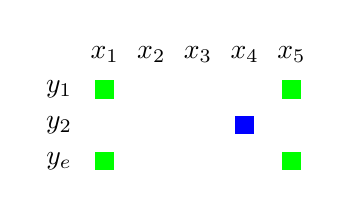
\begin{tikzpicture}
  \matrix
  {
    & \node{$x_1$}; & \node{$x_2$}; & \node{$x_3$}; & \node{$x_4$}; &
    \node{$x_5$}; \\
    \node{$y_1$}; & \node[fill=green]{}; & & & & \node[fill=green]{}; \\
    \node{$y_2$}; & & & & \node[fill=blue]{};  & \\
    \node{$y_e$}; & \node[fill=green]{}; & & & & \node[fill=green]{}; \\
  };
\end{tikzpicture}


\exercise{3.2.1.5}
\paragraph{a.}
$X \times_Z Y = \emptyset$.
\paragraph{b.}
$X \times_Z Y \cong X \times Y$.


\exercise{3.2.1.6}
\paragraph{a.}
$W_1 = \left\{\,\left(\smiley,(0,0,0),((0,0,0),t)\right)\,\vert\,t\in\mathbb{R}\,\right\}$
$W_2 = \left\{\,\left(\smiley,0,(r,0)\right)\,\vert\,r\in\mathbb{R}^3\,\right\}$
\paragraph{b.}
$W_1$ is isomorphic to the set of all events that occured at any time
at MIT's center of mass.  $W_2$ is isomorhic to the set of all events
that occured at the same time as MIT's founding.


\exercise{3.2.1.10}
\paragraph{a.}
appropriate
\paragraph{b.}
appropriate
\paragraph{c.}
debatable\ldots


\exercise{3.2.1.11}
Yes, mother and father are (pullbacks).


\exercise{3.2.1.13}
\begin{tikzcd}
  X \times_Y \{\smiley\}
    \arrow[r]
    \arrow[d]
    \arrow[dr, phantom, "\lrcorner", very near start] &
  \{\smiley\}
    \arrow[d, "y"] \\
  X
    \arrow[r, "f"] &
  Y
\end{tikzcd}


%%% Local Variables:
%%% mode: latex
%%% TeX-master: "exercises"
%%% End:
